\documentclass[aspectratio=169]{beamer}
\usetheme{metropolis}
\usepackage[utf8]{inputenc}
\usepackage[spanish]{babel}
\usepackage{booktabs}
\usepackage{graphicx}
\usepackage{amsmath}
\usepackage{tikz}
\graphicspath{{../../outputs/figures/}}
\definecolor{azul}{HTML}{0072B2}
\definecolor{naranja}{HTML}{E69F00}
\definecolor{verde}{HTML}{009E73}
\definecolor{gris}{HTML}{999999}
\setbeamercolor{frametitle}{bg=azul}
\setbeamertemplate{frame numbering}[fraction]

\title{Winoground: evaluar CLIP en razonamiento composicional}
\subtitle{El retrieval alto no implica composición}
\author{Niels Victor Pacheco Barrios}
\institute{Maestría en Ciencias de la Computación · MCC225 — IA Generativa y Multimodal · 2026-1\\
Segunda Exposición Académica — Trabajo integrador}
\date{}

\begin{document}

% ============ 1. TÍTULO / TRABAJO / MODALIDADES / TAREA ============
\maketitle

\begin{frame}{1 · Trabajo integrador: modalidades y tarea}
  \textbf{Estudiante:} Niels Victor Pacheco Barrios \quad·\quad \textbf{Curso:} MCC225 (2026-1)\\[2pt]
  \textbf{Trabajo:} \emph{Winoground / Evaluating CLIP} — evaluación de un dual-encoder CLIP.
  \vfill
  \begin{columns}[T]
    \column{0.5\textwidth}
    \textbf{Modalidades}
    \begin{itemize}
      \item \textbf{Imagen} (torre visual, ViT).
      \item \textbf{Texto} (torre de lenguaje, transformer).
    \end{itemize}
    \column{0.5\textwidth}
    \textbf{Tarea principal}
    \begin{itemize}
      \item Emparejamiento composicional imagen–texto.
      \item Recuperación (retrieval) sobre pares mínimos.
    \end{itemize}
  \end{columns}
  \vfill
  \centering\footnotesize\textbf{Tesis:} un \emph{Recall@K} alto \alert{no} implica razonamiento composicional.
\end{frame}

% ============ 2. PROBLEMA / MOTIVACIÓN / DATOS / ÉXITO ============
\begin{frame}{2 · Problema, motivación, datos y criterio de éxito}
  \begin{columns}[T]
    \column{0.54\textwidth}
    \textbf{Problema.} ¿CLIP \emph{entiende} la escena o solo \emph{empareja} conceptos?\\[4pt]
    \textbf{Motivación.} Winoground usa \emph{pares mínimos}: 2 imágenes y 2 captions con las
    \textbf{mismas palabras en distinto orden}. Distinguirlos exige saber \emph{quién hace qué a quién},
    no reconocer objetos sueltos.
    \column{0.46\textwidth}
    \textbf{Datos disponibles}
    \begin{itemize}
      \item Winoground: \textbf{400} pares mínimos.
      \item Etiquetas: \emph{Object}, \emph{Relation}, \emph{Both}.
    \end{itemize}
    \textbf{Criterio de éxito}
    \begin{itemize}
      \item \textbf{group score} $>$ azar $= 1/6 \approx \mathbf{0.167}$.
      \item Referencia humana $\approx 0.855$.
    \end{itemize}
  \end{columns}
  \vfill
  \centering\footnotesize El azar del group es $1/6$ (no $1/16$): de las $4!=24$ ordenaciones de las 4 similitudes, solo 4 aciertan.
\end{frame}

% ============ 3. ARQUITECTURA + COMPARACIÓN ============
\begin{frame}{3 · Arquitectura: dual-encoder CLIP vs.\ cross-encoder}
  \small
  \begin{center}
  \begin{tabular}{lll}
    \toprule
     & \textbf{Dual-encoder (CLIP)} & \textbf{Cross-encoder (BLIP/fusión)} \\
    \midrule
    Alineamiento    & tardío, 1 vector global/modalidad & profundo, token-a-token (cross-attention) \\
    Costo           & barato, escala a retrieval masivo & caro, no escala a galería grande \\
    Tipo de error   & falla composición (orden/relación) & mejor grounding, mejor composición \\
    Interpretab.    & solo similitud coseno global & mapas de atención cruzada \\
    Pertinencia     & \textbf{elegido}: reproducible en CPU/MPS & propuesto como contraste/mejora \\
    \bottomrule
  \end{tabular}
  \end{center}
  \vfill
  \footnotesize\textbf{Decisión (ADR 0001):} evaluar el dual-encoder (motor OpenCLIP, C10) como sujeto principal
  --- ligero, determinista, defendible --- y usar la fusión profunda (C5) / atención crossmodal (C8) como
  \emph{marco de contraste} que explica \emph{por qué} el dual-encoder falla la composición.
\end{frame}

% ============ 4. TRANSFORMER Y ATENCIÓN ============
\begin{frame}{4 · Transformer y atención, conectados al modelo}
  \begin{columns}[T]
    \column{0.5\textwidth}
    \footnotesize
    \textbf{Del texto/imagen a tokens.} Entrada $\to$ tokens $\to$ \emph{embeddings} + codificación de \emph{posición}
    (imagen: parches ViT; texto: subpalabras).\\[4pt]
    \textbf{Atención producto-punto escalada:}
    \[
      \mathrm{Attn}(Q,K,V)=\mathrm{softmax}\!\left(\frac{QK^{\top}}{\sqrt{d}}\right)V
    \]
    $Q$ (consulta), $K$ (clave), $V$ (valor); pesos = afinidad token-token.\\[4pt]
    Costo \textbf{$O(n^2)$} en la longitud de secuencia $n$.
    \column{0.5\textwidth}
    \footnotesize
    \textbf{Self- vs cross-attention.}
    \begin{itemize}
      \item \emph{Self}: tokens atienden dentro de \textbf{una} modalidad.
      \item \emph{Cross}: tokens de imagen atienden a los de texto (y viceversa) $\Rightarrow$ grounding.
    \end{itemize}
    \textbf{En CLIP (dual-encoder):} solo \textbf{self-attention} dentro de cada torre; los tokens de imagen
    y de texto \alert{nunca} interactúan directamente --- cada modalidad colapsa a un vector global antes de compararse.
    \par\vspace{3pt}
    \alert{Sin cross-attention $\Rightarrow$ sin alineamiento token-a-token $\Rightarrow$ composición débil.}
  \end{columns}
\end{frame}

% ============ 5. EVIDENCIA EXPERIMENTAL ============
\begin{frame}{5 · Evidencia experimental (motor C10 / pipeline Winoground)}
  \begin{columns}[c]
    \column{0.46\textwidth}
    \scriptsize
    \begin{tabular}{lcc}
      \toprule
      Métrica & Valor & Azar \\
      \midrule
      text score  & 0.3475 & 0.25 \\
      image score & 0.110  & 0.25 \\
      \textbf{group score} & \alert{0.075} & 0.167 \\
      \midrule
      R@5 (t2i)   & 0.667 & --- \\
      R@10 (t2i)  & 0.774 & --- \\
      \bottomrule
    \end{tabular}
    \par\vspace{4pt}
    \footnotesize ViT-B-32/laion2b, $N=400$. IC bootstrap 95\% del group $[0.05,\,0.10]$:
    \textbf{entero por debajo del azar}. Humano $\approx 0.855$.
    \column{0.54\textwidth}
    \centering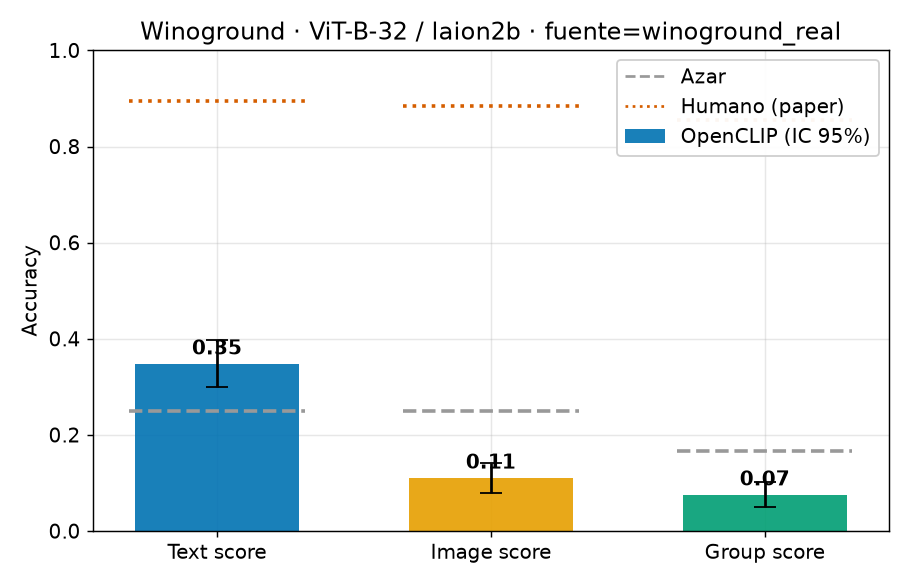
\includegraphics[height=0.72\textheight]{scores_vs_chance.png}
  \end{columns}
  \vfill
  \centering\footnotesize \textbf{Retrieval alto} ($R@10{=}0.774$) con \alert{group muy por debajo del azar} ($0.075$ vs $0.167$): retrieval $\ne$ composición.
\end{frame}

% ============ 6. ANÁLISIS DE ERRORES ============
\begin{frame}{6 · Análisis de errores: aciertos, fallos y límites}
  \begin{columns}[c]
    \column{0.5\textwidth}
    \centering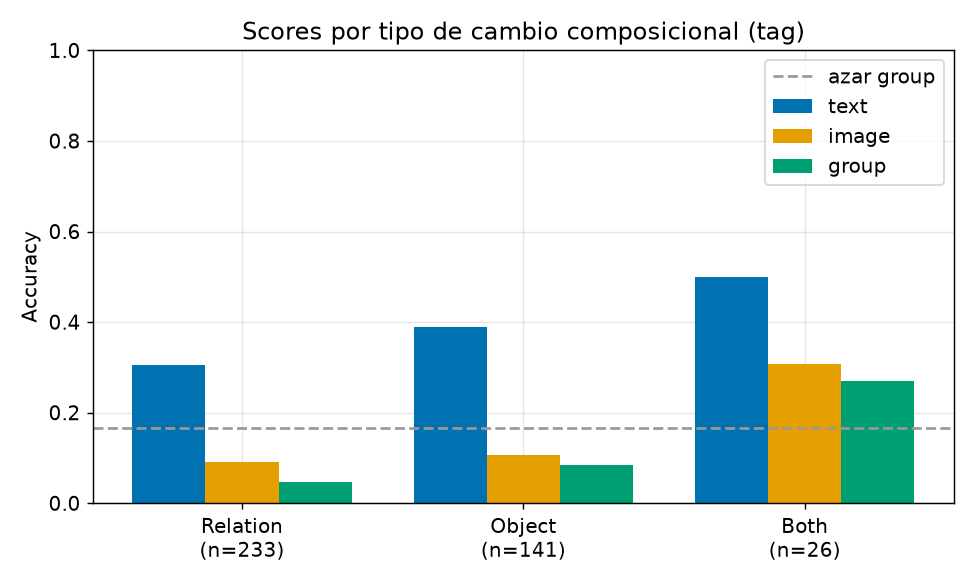
\includegraphics[height=0.66\textheight]{by_tag.png}
    \column{0.5\textwidth}
    \footnotesize
    \textbf{Correctos.} El modelo detecta bien objetos $\Rightarrow$ retrieval y text score sobre el azar.\\[4pt]
    \textbf{Fallos por tag (group):}
    \begin{itemize}
      \item \textbf{Relation}: \alert{0.047} ($n{=}233$) --- peor: fallo de \emph{vinculación} (quién con quién).
      \item Object: 0.085 ($n{=}141$).
      \item Both: 0.269 ($n{=}26$) --- las dos imágenes difieren más.
    \end{itemize}
    \textbf{Limitaciones.} El group bajo mezcla fallo composicional con ítems ambiguos (Diwan et al.);
    métricas estrictas sensibles a empates.
  \end{columns}
\end{frame}

% ============ 7. ACTIVIDAD 5 ============
\begin{frame}{7 · Actividad 5: confiabilidad, explicabilidad, robustez, riesgos}
  \begin{columns}[c]
    \column{0.42\textwidth}
    \centering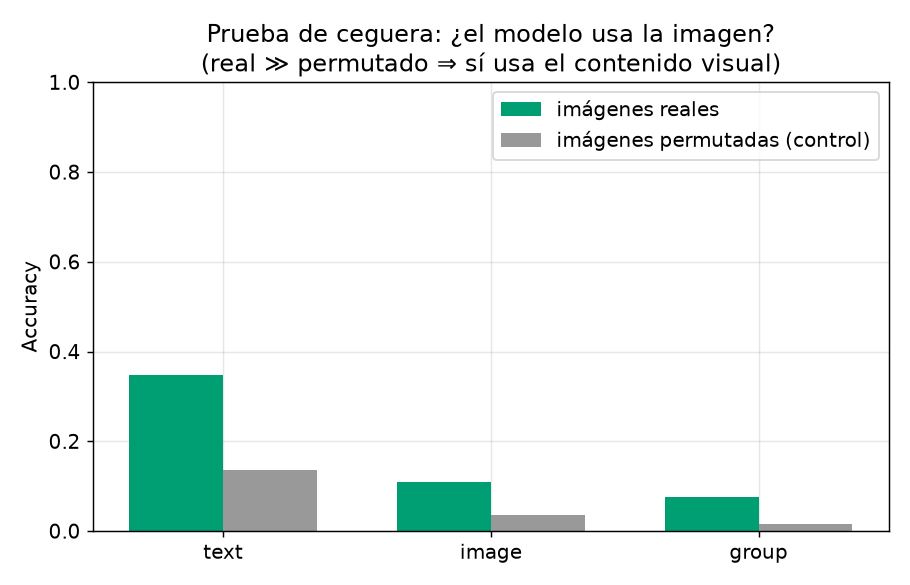
\includegraphics[width=\linewidth]{blindness.png}
    \column{0.58\textwidth}
    \footnotesize
    \textbf{Confiabilidad.} Scorer validado contra los scores oficiales \texttt{clip.jsonl}
    (0.3075/0.105/0.08): coincidencia exacta. IC bootstrap reportados.\\[3pt]
    \textbf{Explicabilidad (prueba de ceguera).} Permuto las imágenes y recalculo: los scores
    caen de $0.3475/0.110/0.075$ a \textbf{$0.135/0.035/0.015$} ($\approx$ azar).
    $\Rightarrow$ el modelo \textbf{sí usa la imagen}; su límite es \emph{composicional}, no perceptivo.\\[3pt]
    \textbf{Robustez.} Escalar tamaño/datos no ayuda: group $0.075\!\to\!0.073\!\to\!0.085$;
    el text incluso baja ($0.3475\!\to\!0.2975\!\to\!0.2875$).\\[3pt]
    \textbf{Riesgos/sesgos.} R@K alto puede \emph{sobrevender} comprensión; sesgo de bolsa-de-conceptos
    ignora orden y relaciones.
  \end{columns}
\end{frame}

% ============ 8. PLAN DE CIERRE ============
\begin{frame}{8 · Plan de cierre hacia la defensa final}
  \footnotesize
  \setlength{\itemsep}{1pt}
  \textbf{Por implementar}
  \begin{itemize}\itemsep1pt
    \item Evaluar un \textbf{cross-encoder profundo real} (BLIP/MMBT, C5), más allá del
    \emph{re-ranker-lite} ya probado (§12 del notebook): interacción cruzada real (C6).
    \item Versionar embeddings (DVC) para reproducibilidad total de datos.
  \end{itemize}
  \vspace{-3pt}\textbf{Por validar}
  \begin{itemize}\itemsep1pt
    \item Ampliar a más prompts / \emph{prompt ensembles} y más checkpoints (C10).
    \item Confirmar estabilidad de los IC con más rondas de bootstrap.
  \end{itemize}
  \vspace{-3pt}\textbf{Por corregir / matizar}
  \begin{itemize}\itemsep1pt
    \item Separar fallo composicional de ítems ambiguos (Diwan et al.).
    \item El set curado offline es un \emph{proxy}; priorizar acceso al benchmark gated.
  \end{itemize}
  \vspace{1pt}
  \centering\scriptsize Hipótesis abierta: que un cross-encoder \emph{profundo} cierre la brecha composicional que el re-ranker-lite no cerró.
  \par\vspace{1pt}
  {\scriptsize\color{gris} Trabajo individual. Se usó asistencia de IA generativa; las definiciones de métrica se verificaron contra el paper de Winoground y el scorer oficial.}
\end{frame}

\end{document}
